\setchapterpreamble[u]{\margintoc}
\glsresetall % reset glossary

\chapter{Design of real-size aeronautical wing structures} \label{chap:07}

Ultralight trusses are a good design candidate for the design of innovative aerostructures thanks to their superior aeroelastic properties and stiffness-to-weight ratio \sidecite{cramer_elastic_2019}. These structures represent a natural application case for the discussed optimization formulations until that point. Opgenoord \sidecite{opgenoord_aeroelastic_2018, opgenoord_design_2019} proposed a two-step sequential optimization algorithm to reduce the weight of a truss wing. Firstly, a ground structure with different nodal densities based on the stress field of the structure is generated and secondly, the cross-sectional areas are found using a sizing optimization algorithm that takes into account stress, local buckling, and aeroelastic constraints. Shahabsafa \sidecite{shahabsafa_novel_2018} decided, instead, to tackle all the difficulties of the problem using a set of discrete cross-sectional areas and a sizing \gls{milo} algorithm. In these studies, the adoption of a sizing optimization algorithm simplifies the numerical complexities associated with the problem. However, by solely focusing on modifying the component sizes, the opportunity to optimize the overall truss topology is missed, limiting the potential for further weight savings. Additionally, no one of these study evalued the febrivcabiliry of the proposed design. it is here that the modularity cound be beneficial.

In the precedent chapters we focused on the developement of optiization methods for monolitich and modular structures, and we applied them to two and three dimensional academic load cases. Here we want to validate the proposed optimization algorithms by testing them on real world engineering problem in the aeronautic domain. First, to assess the computational efficiency and to validate the strategy proposed in \chpref{chap:04} on a large-scale structure, we optimize a monolitich three-dimensional wingbox test case based on the \acrfull{crm} with multiple load cases and for two discretization refinement. Later, we put the modular algorithm presented in \chpref{chap:06} on a drone-sized wing based on a extruded NACA 0012 profile.

The optimizations presented in this section are performed on a notebook equipped with an Intel\textsuperscript{\textregistered} Core™ i5-9400H Processor @ \qty{2.50}{GHz} (4 cores) and \qty{16}{GB} of RAM. 

\section{3D CRM wingbox with multiple load cases}
In this section, the proposed strategy is used to optimize a real-size wingbox, to validate its ability to work on large, three-dimensional structures with more candidate members compared to the precedent test cases. The structure is based on the jig (undeformed) shape of the wingbox of the NASA \gls{crm} \sidecite{brooks_benchmark_2018}. The structure is submitted to three different load cases: +2.5 g maneuver (LC\_1), -1 g maneuver (LC\_2), and cruise with gust +1.3 g (LC\_3). The nodes of the bounding volume and the loads used are provided by Fakhimi \etal \sidecite{fakhimi_discrete_2021}, where a detailed discussion on how they are evaluated can be found. The ground structure of the test case is presented in \figref{fig:07_crm315_x0}. Additionally, the load cases and the starting point, of all the presented test cases are available in the reference data set \sidecite{enrico_stragiotti_truss_2023}.

The material used for the optimization is an aluminum alloy with Young's modulus of \qty{69}{\GPa}, density of \qty{2.7}{\gram/\cm^3}, and yield stress equal to $\pm$\qty{270}{\MPa} (see \tabref{tab:07_CRM_mat}). To ensure a conservative design, we incorporated safety factors (\textit{sf}) associated with each load case. These safety factors are integrated into the formulation by reducing the maximum stress and buckling allowables by factors of 1.5, 1.5, and 2.67 for the three considered load cases, respectively. The cross-sections are assumed circular with the cross-sectional buckling parameter $s = \pi E/4$. The optimization is carried only on the wingbox, the internal structure of the wing, and there is no influence of the skin on the optimization.
\begin{margintable}
    \small
    \centering
    \begin{tabular}{cc}
    \toprule
    \textbf{Parameter}        & \textbf{Value} \\ \midrule
    $E$              & \qty{69}{GPa}     \\
    $\sigma_\text{c}, \sigma_\text{t}$ & $\pm $\qty{270}{MPa} \\
    $\rho$              & \qty{2.7}{\gram\per\cubic\centi\metre}   \\
    \bottomrule
    \end{tabular}
    \caption{Material data used for the CRM optimization.}
    \label{tab:07_CRM_mat}
\end{margintable}

The optimizations are performed using the Python package CVXPY 1.2.2 \sidecite{diamond_cvxpy_2016} with the ECOS 2.0.7 \sidecite{domahidi_ecos_2013} solver to solve the relaxed \gls{lp} Problem \eqref{eq:04_optim_no_constr_lp}. The \gls{nlp} Problem \eqref{eq:04_optim_complete} is solved using cyipopt \sidecite{Moore_Mechmotum}, a Python wrapper for IPOPT 3.14.11 \sidecite{wachter_implementation_2006}, a large-scale nonlinear optimization package using PARDISO 6.0 \sidecite{alappat_recursive_2020} as the linear solver. The Jacobian and the Hessian of the Lagrangian of the \gls{nlp} step are calculated at every optimization iteration to allow faster convergence. As every state variable of the optimization is independent of the others, these responses are derived analytically and will not be detailed there. The stopping criterion used for the \gls{slp} and \gls{nlp} optimisations are $\norm{\Delta \vect{x}}_\infty \leq \text{tol}_{slp}  \text{, and } \norm{\Delta_{\text{NLP}}}_\infty \leq \text{tol}_{nlp}$, with $\text{tol}_{slp}=10^{-6}$ and $\text{tol}_{nlp}=10^{-4}$ respectively. $\Delta_{\text{NLP}}$ represents the scaled \gls{nlp} error, a more comprehensive value used by IPOPT to take into account the optimality of the solution and the constraints violation. The reinitialization magnitude parameter $\vect{\phi}$ is set up using \eqref{eq:04_phi} \marginnote{\eqref{eq:04_phi} reads: $$\phi_n = \phi_{n-1}^\beta \quad \forall n \in [1,\dots,n_{\text{max}}],$$ with $\phi_0=0.8$ and $\beta=2$.}, leading to $\vect{\phi} = \left[ 0.8000, 0.6400, 0.4096, 0.1677, 0.0281 \right]$ for the five reinitialization calls of 2S-5R. The full list of parameters used to set up the variable scaling, the SLP optimization, the reinitialization, and the NLP optimization is the same used in \chpref{chap:04} listed in \tabref{tab:04_param}.

\subsection{Advanced thresholding}
As the \gls{crm} is a large and thin structure that presents a noticeable difference in load magnitude between the tip and the root of the wingbox, the quantities of interest of the optimization span different orders of magnitude (from \unit{m^2} to \unit{mm^2}, and\marginnote{\eqref{eq:04_thr} reads: $$a_i<a_{\text{thr}} \; \forall i, \text{ with }a_{\text{thr}} = \chi \; \max(\tilde{\vect{a}}^*)$$} from \unit{MN} to \unit{N}). For that reason, the choice of the cross-sectional area threshold value $\chi$ defined in \eqref{eq:04_thr} and used to simplify the initial \gls{nlp} ground structure is crucial. Taking a high value (such as $\chi = 10^{-4}$, restraining the solution from \unit{m^2} to \unit{cm^2}) would mean possibly canceling out bars fundamental for the nodal force equilibrium in the less loaded part of the wing (wing tip and the central part of the wing's sections near the root). By contrast, a low value (such as $\chi=10^{-9}$) would permit the correct simulation of the mechanical response of the structure, but it would lead to a very high number of candidate bars and, thus, longer optimizations and convergence difficulty for the \gls{nlp} phase. For that reason, $\chi$ is set to an average value ($\chi=10^{-6}$), eliminating all the bars under the value $a_{\text{thr}}=\chi \; \max(\vect{a})$, but an additional check is performed before proceeding to the thresholding. The bars under the threshold $a_{\text{thr}}$ are sorted in ascending order of cross-sectional area and, starting from the smallest one, we iteratively check via a \gls{fea} that the difference between the force and displacement fields before and after the bar removal is below than a certain bound. In the present study we used the following: $\norm{\Delta q}_{\infty}<\qty{10}{N}$ and $\norm{\Delta U}_{\infty}<\qty{1}{cm}$.
\subsection{Numerical optimization}    
    \begin{figure*}
        \centering
        \subcaptionbox{\label{fig:07_crm315_x0}}{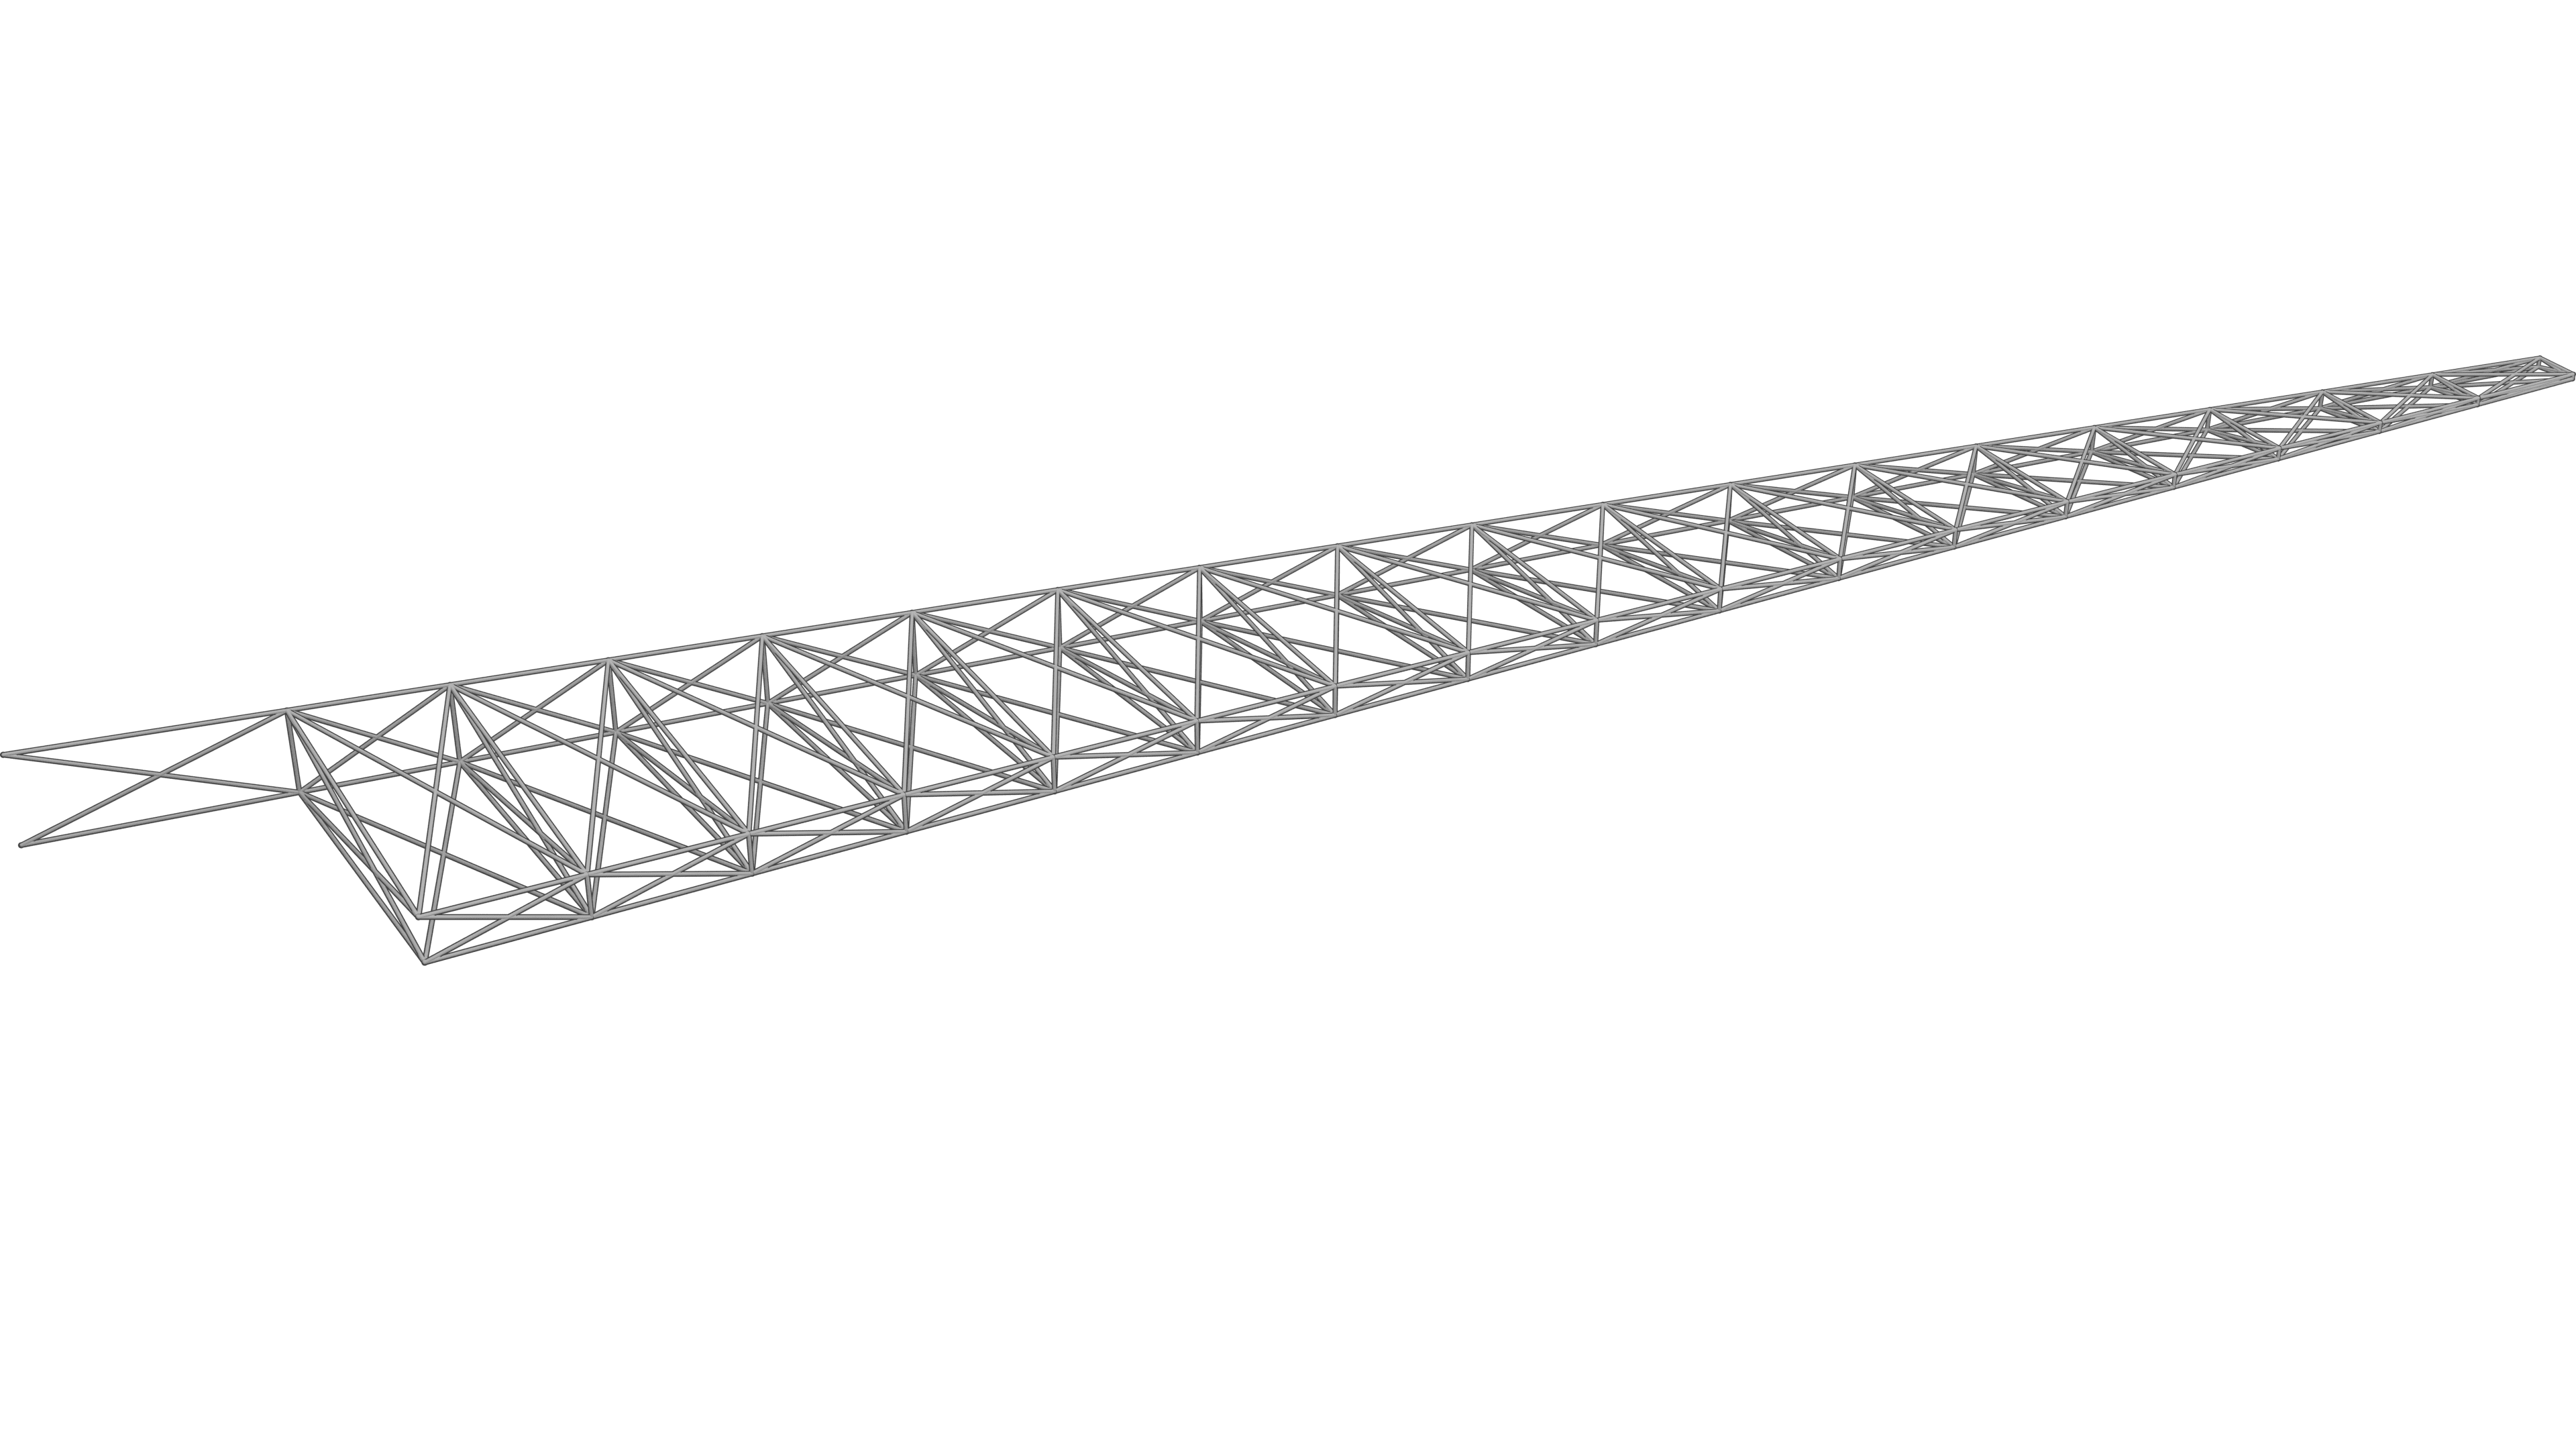
\includegraphics[width=0.45\linewidth]{figures/07_aeronautic/14a_00_Topology_x0_iso.png}}
        \bigskip
        \subcaptionbox{\label{fig:07_crm2317_x0}}{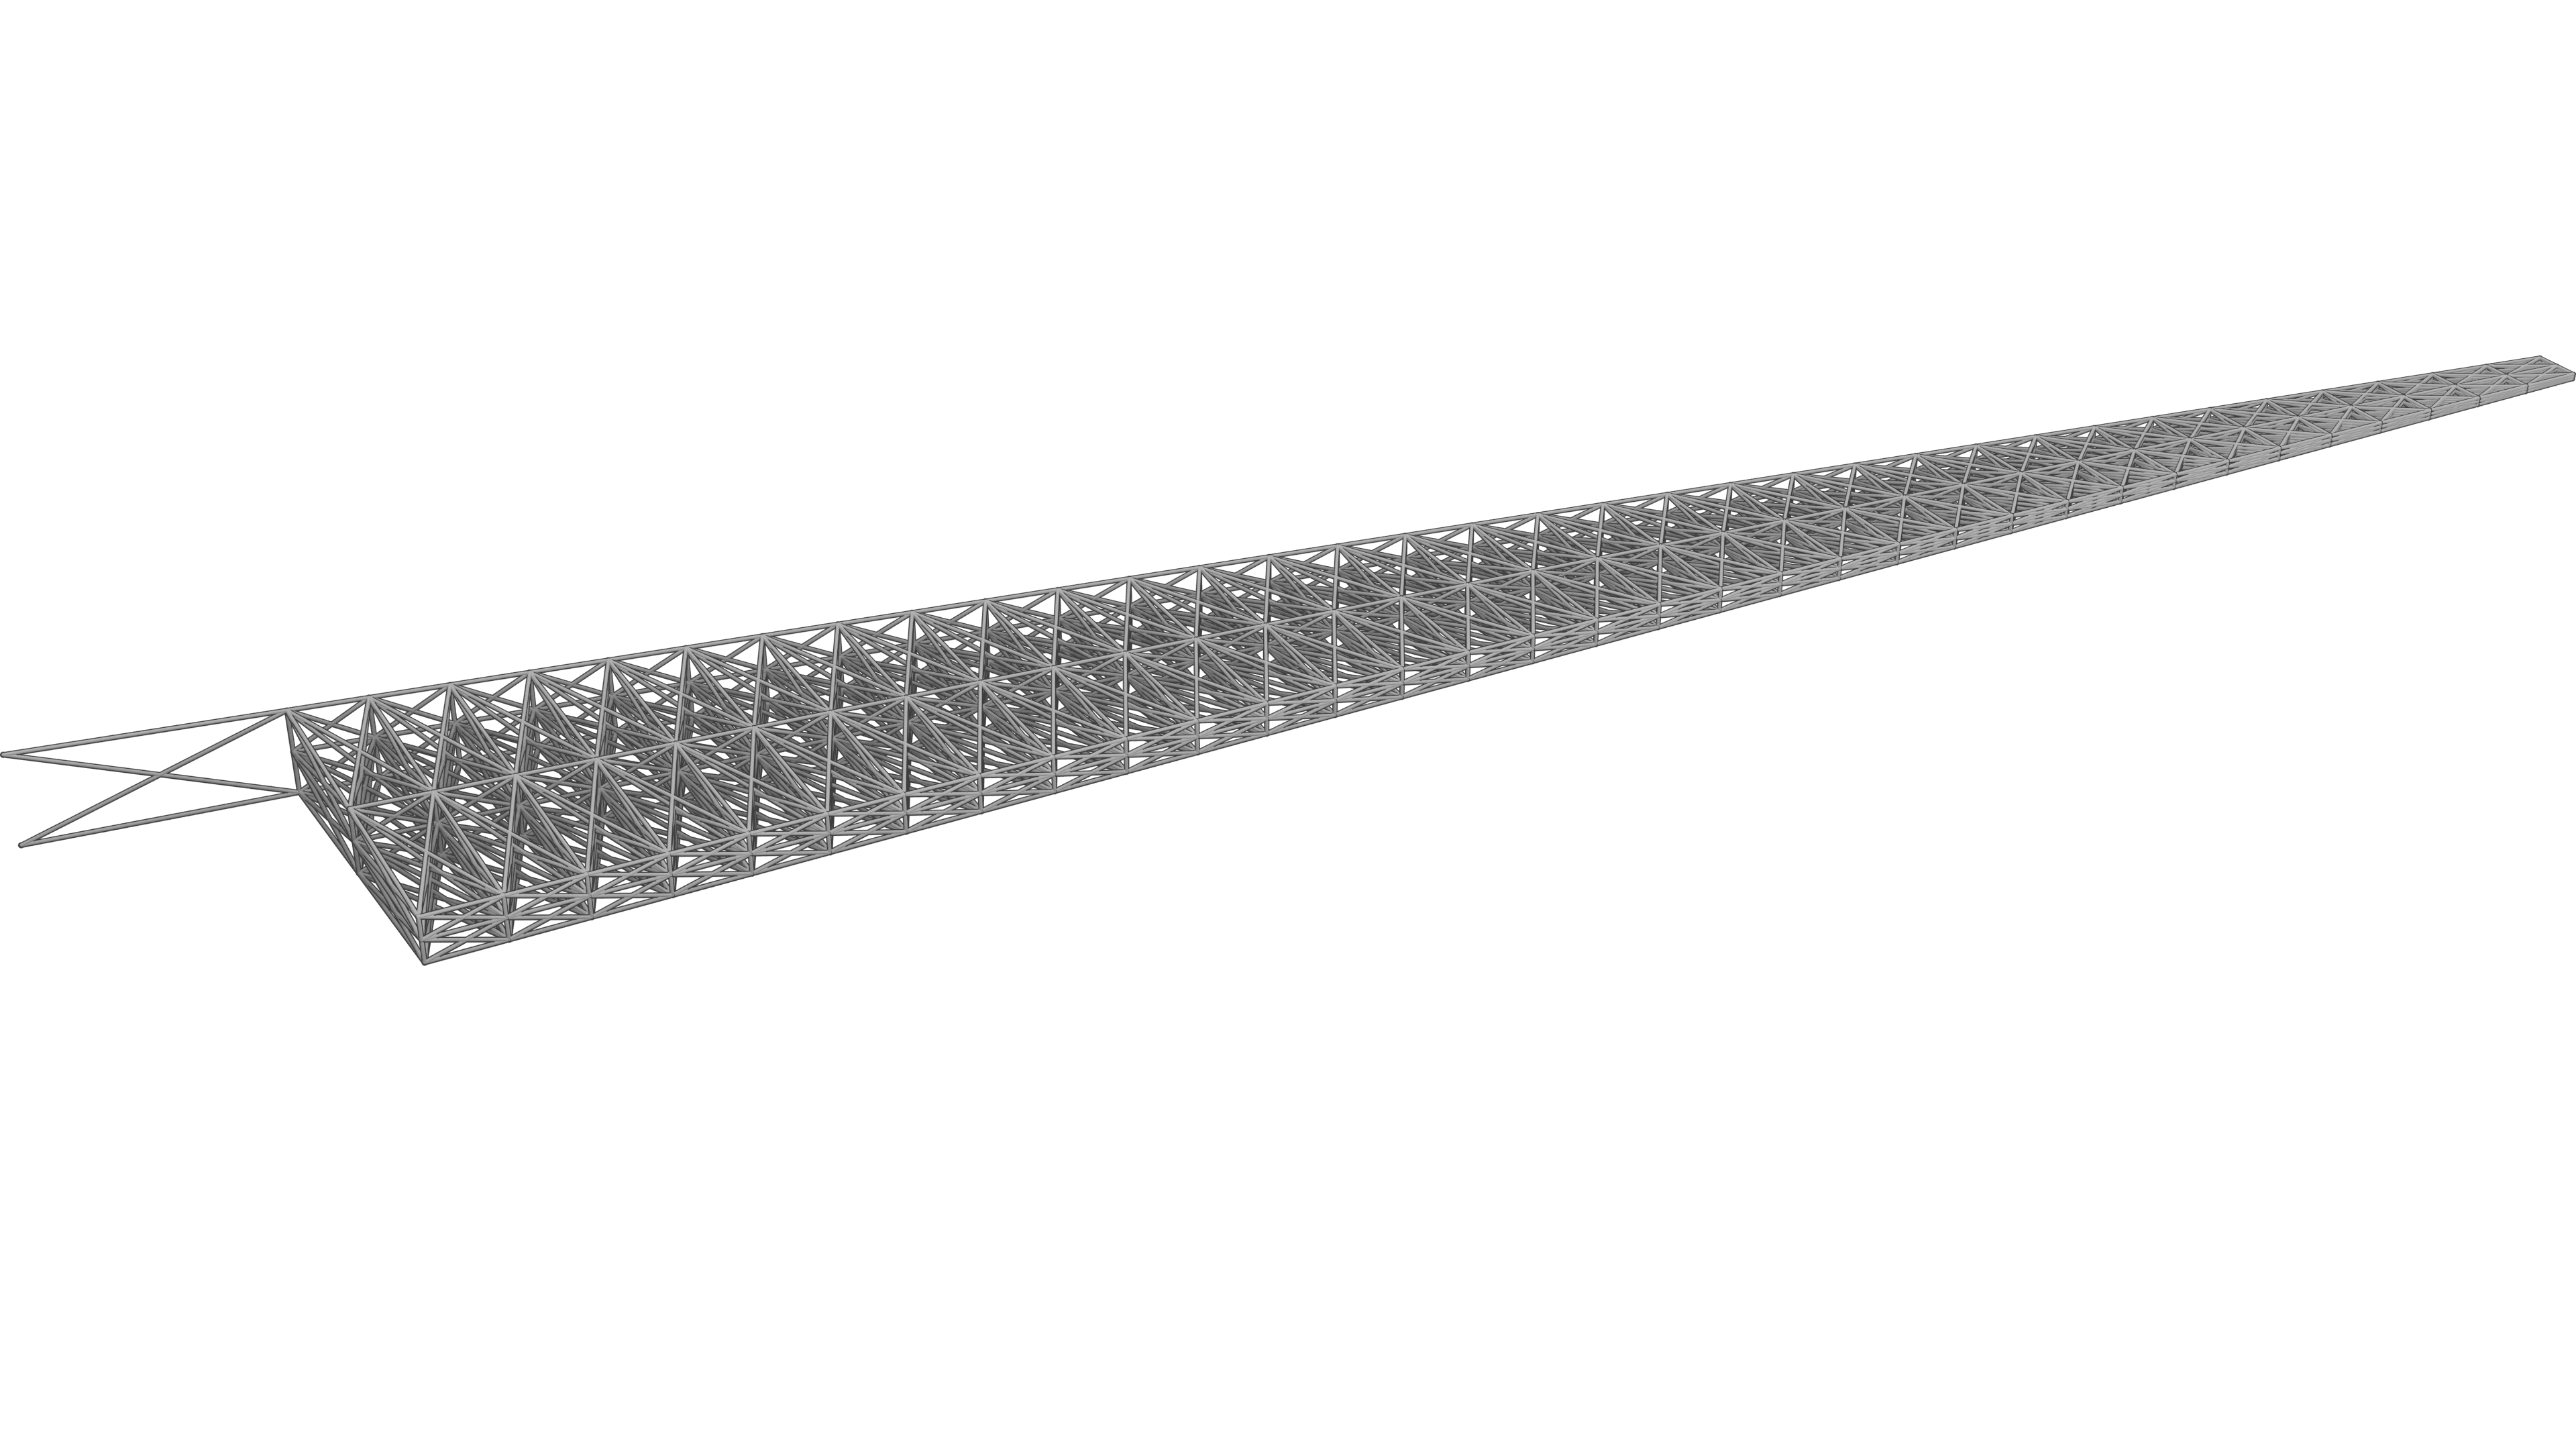
\includegraphics[width=0.45\linewidth]{figures/07_aeronautic/14b_00_Topology_x0_iso 2370.png}}
        \caption{(a) Ground structure of the CRM-315 test case; (b) Ground structure of the CRM-2370 test case. The cross-sectional areas shown in the two sub-figures represent the starting point of the optimizations.}
        \label{fig:07_crm}
    \end{figure*}
    
    \begin{figure}
        \centering
        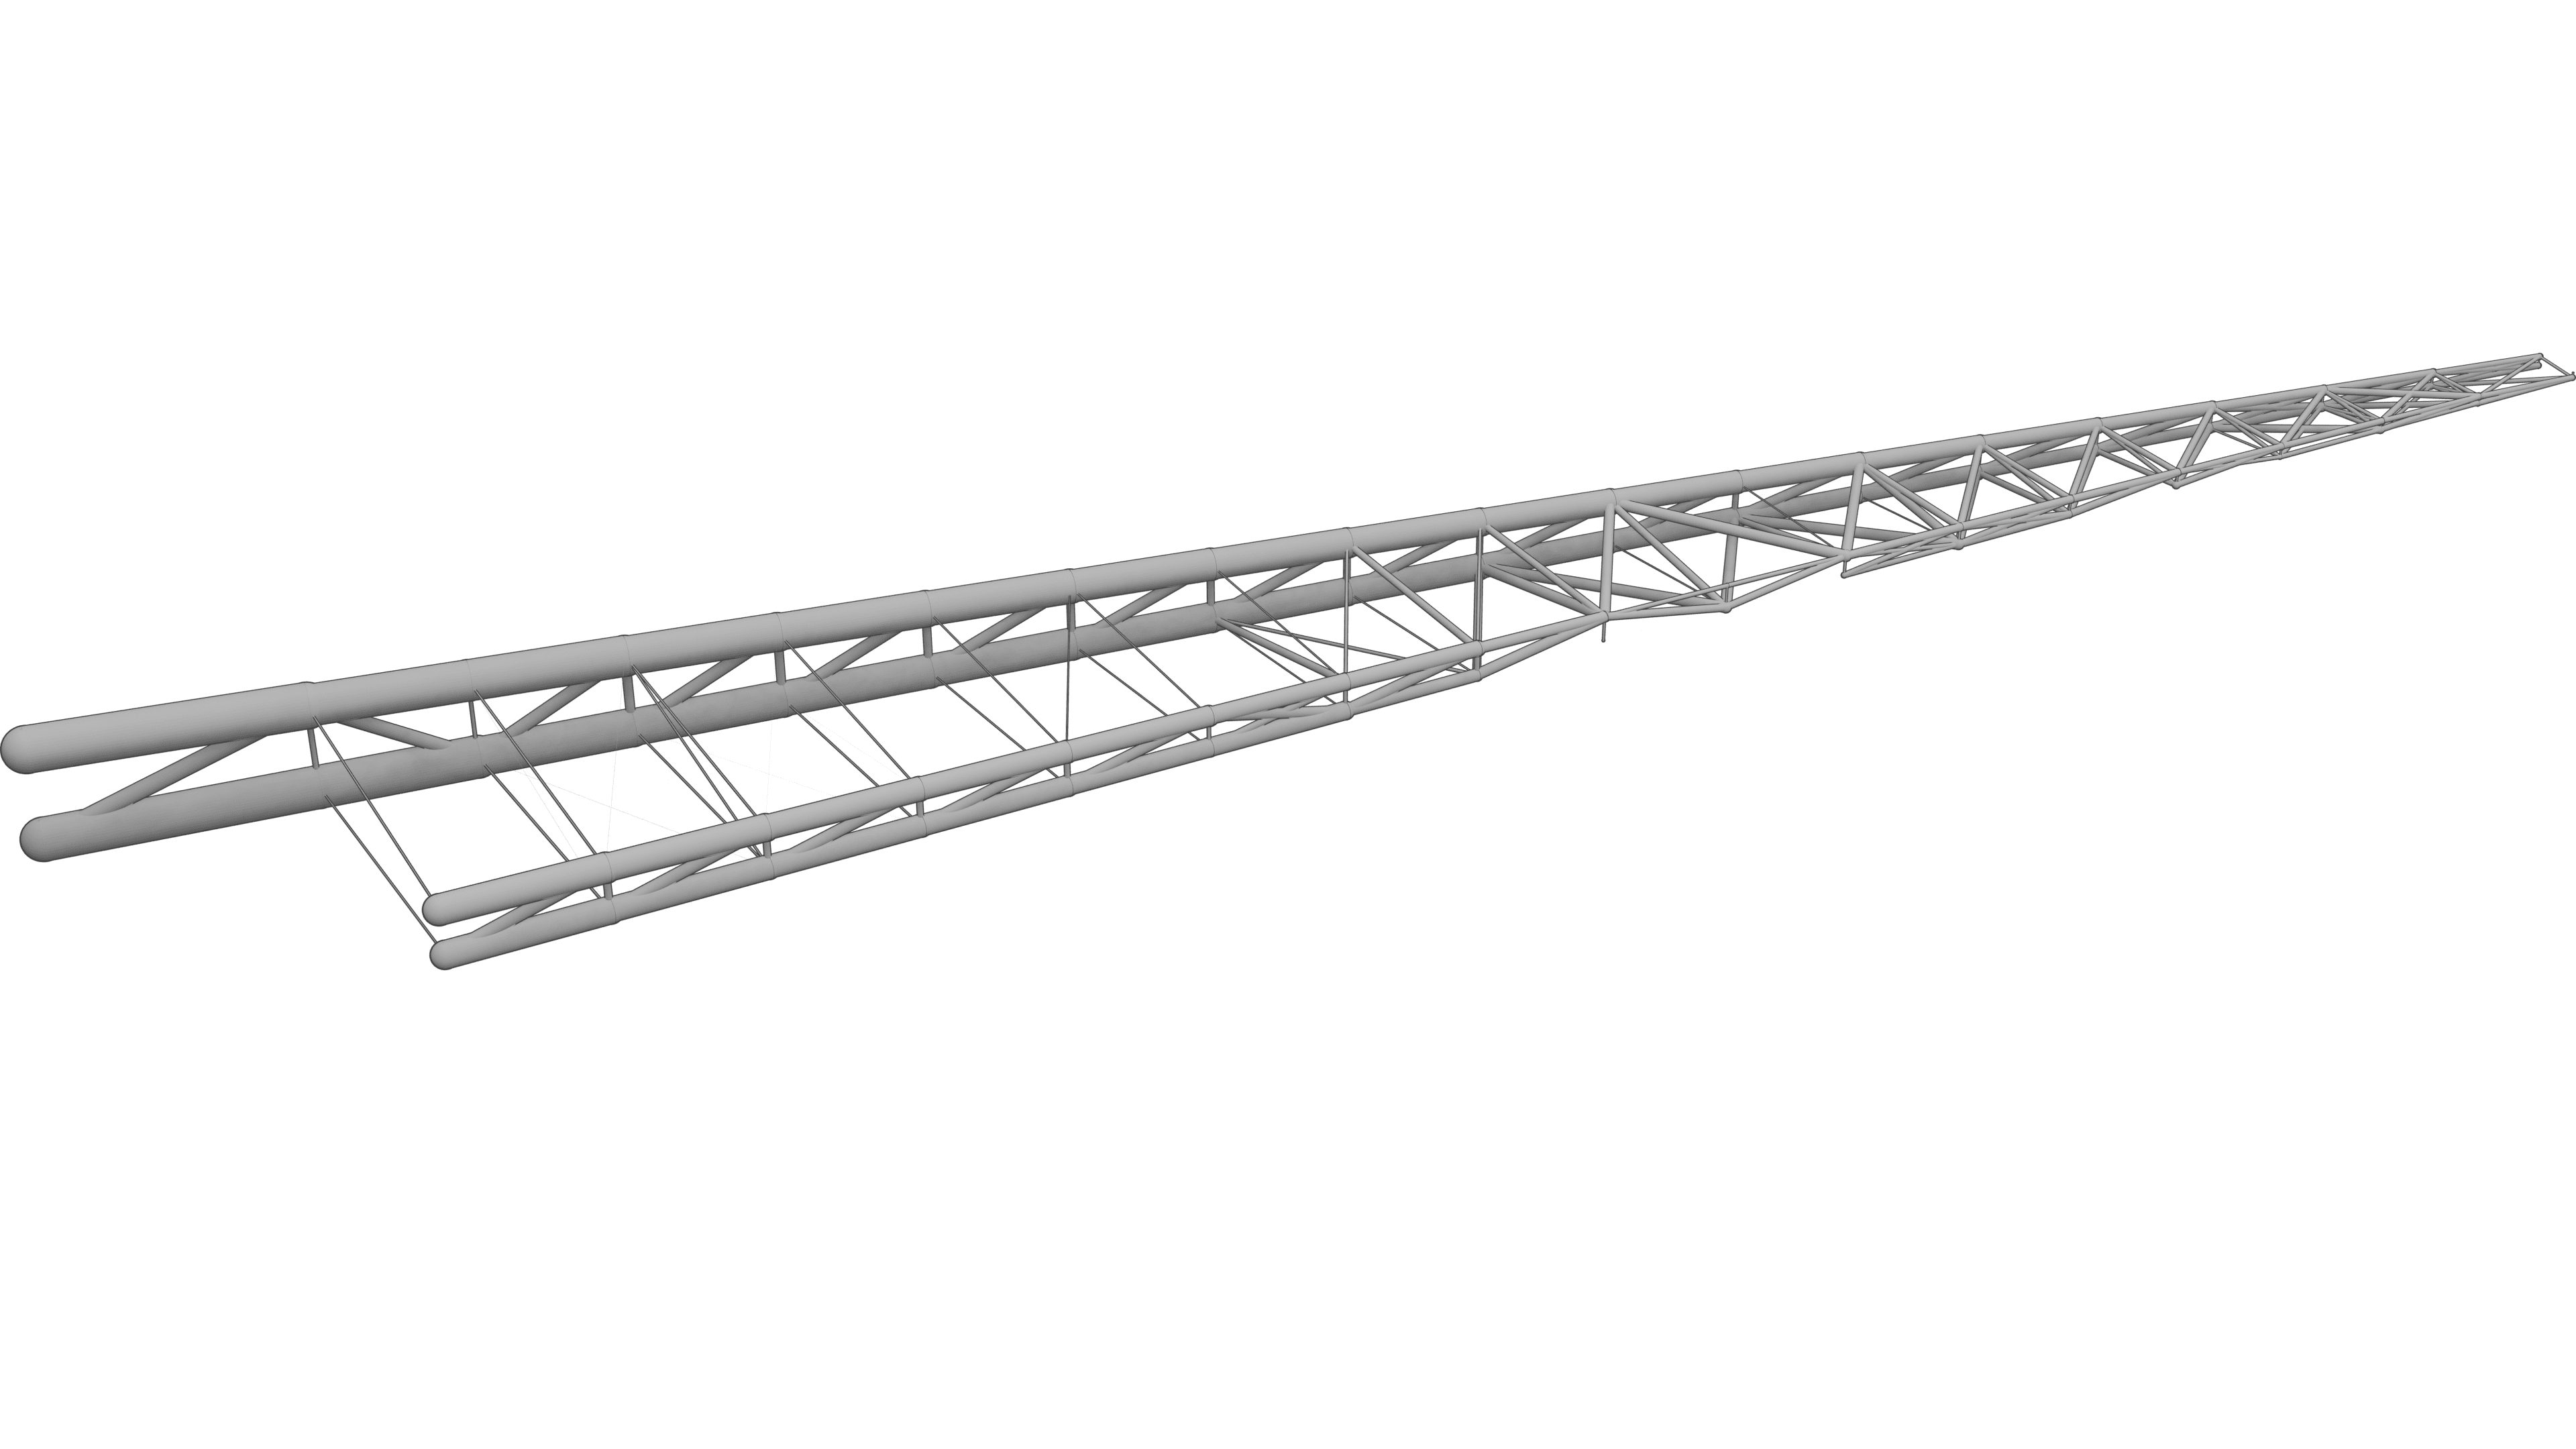
\includegraphics[width=0.8\linewidth]{figures/07_aeronautic/15_04_Topology_NLP_iso.png}
         \caption{Optimized topology of the CRM-315 with 257 active bars.}
        \label{fig:07_crm315}
    \end{figure}
    
    Two different discretizations are considered for the optimization. The proposed algorithm is firstly tested on the same ground structure provided by Fakhimi \etal \sidecite{fakhimi_discrete_2021}, composed of $N_{\text{el}}=315$ candidate members (CRM-315). The second discretization is obtained by refining the 315-bar ground structure, evaluating the midpoints of every member, and connecting them with first-order connectivity. We obtain $N_{\text{el}}=2370$ candidate members (CRM-2370). The loads and the boundary conditions are applied on the same nodes of the ground structure for the two studied ground structures. The cross-sectional areas of the starting point of the CRM-315 and the CRM-2370 are set to \qty{0.0001}{m^2} and they are shown in \figref{fig:07_crm}. Only one single start point is used for these two examples as the proposed two-step strategy with reinitialization already proved in \chpref{chap:04} to reduce the starting point influence on the optimization result. The resolution algorithm used is 2S-5R. The numerical results of the optimization for the two different discretizations are reported in \tabref{tab:07_wing-res}. 
    
    The optimized CRM-315 structure shows a mass of \qty{21.342}{\tonne}, a \qty{27.01}{\%} reduction compared to the solution with discrete cross-section areas found by Fakhimi \etal \sidecite{fakhimi_discrete_2021} (\qty{29.238}{\tonne}). Other than the substantial difference in the modelization of the cross-section areas, the mass reduction could be explained by the fact that the proposed algorithm has a zero lower bound on cross-sectional areas, thus permitting the topology of the structure to change: the 2S-5R solution shows 257 active bars out of 315 at convergence (see \figref{fig:07_crm315}). In contrast, the \gls{milo} problem solved by Fakhimi \etal \cite{fakhimi_discrete_2021} is employed as a sizing optimization algorithm with fixed topology (and thus 315 active members in the optimized design). A more detailed comparison could not be performed as the authors did not share the values of the cross-sectional areas of their solution. 
    
    The volume fraction of the solution is \qty{1.313}{\percent} and the minimum slenderness ratio $\lambda$ (ratio between the length and the radius of gyration of the bar) of a bar is 14.96, which is compatible with the truss modelization used to discretize the wingbox volume. The execution time of the optimization is \qty{19}{s} for the \gls{slp} step and \qty{128}{s} for the \gls{nlp} step, for a total of \qty{147}{s} on a regular notebook, compared to the over four days of optimization of Fakhimi \cite{fakhimi_discrete_2021} on a desktop workstation. The iteration history curves of the optimization are plot in \figref{fig:07_c2}a, in which we notice the sharp volume increase due to the reinitialization heuristic in the \gls{slp} step. \figref{fig:07_c2}b shows invece the constaint violation curves for the NLP phase. The starting point coming from the relaxed \gls{slp} step violates the stress and buckling constraints as the predicted force field does not account for kinematic compatibility, necessary due to the multiple loading condition of this test case. From the graph we can notice how the kinematic  compatibility constraint is extremely hard to satisfy.

    \begin{table}
        \small
        \centering
        \begin{tabular}{ccc}
        \toprule
        \textbf{Quantity} & \textbf{CRM-315} & \textbf{CRM-2370} \\ \midrule
        N$_{\text{el}}$          & 315               & 2370               \\
        N$_{\text{opt}}$           & 257                  &  1127              \\
        V [\unit{\meter^3}]             &  7.90                 &  7.44             \\
        V [\unit{\%}]             &   \qty{1.309}{\%}                & \qty{1.232}{\%}               \\
        Mass [\unit{\tonne}]               &   21.342                & 20.092     \\
        a$_{\text{max}}$ [\unit{\meter^2}]           &  0.198                 & 0.208              \\
        C$_\text{LC\_1}$ [\unit{\mega \joule}]                &  3.23                 &  3.17              \\
        C$_\text{LC\_2}$ [\unit{\mega \joule}]                &   1.28                &  1.27              \\
        C$_\text{LC\_3}$ [\unit{\mega \joule}]                &   0.76                &  0.74              \\
        t [\unit{\second}]                & 147                  & 3189   \\ \bottomrule            
        \end{tabular}
        \caption{Numerical results of the optimization of the CRM with two different ground structures.}
        \label{tab:07_wing-res}
    \end{table}

    \begin{figure*}
        \centering
        \subcaptionbox{}{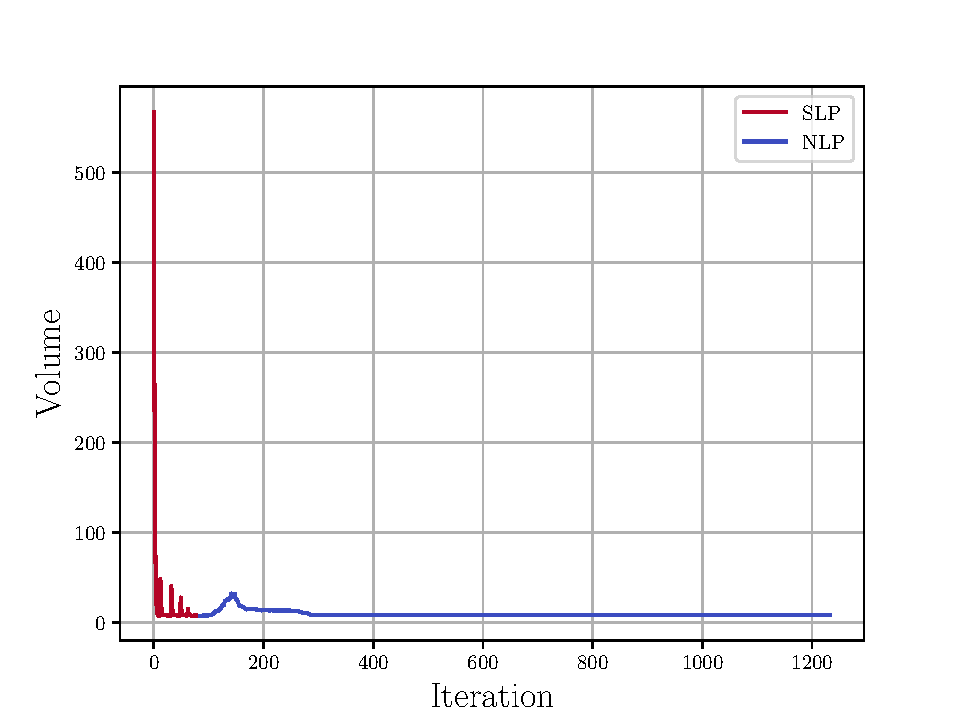
\includegraphics[width=0.49\linewidth]{figures/07_aeronautic/19a_v_hist_315.pdf}}
        \bigskip
        \subcaptionbox{}{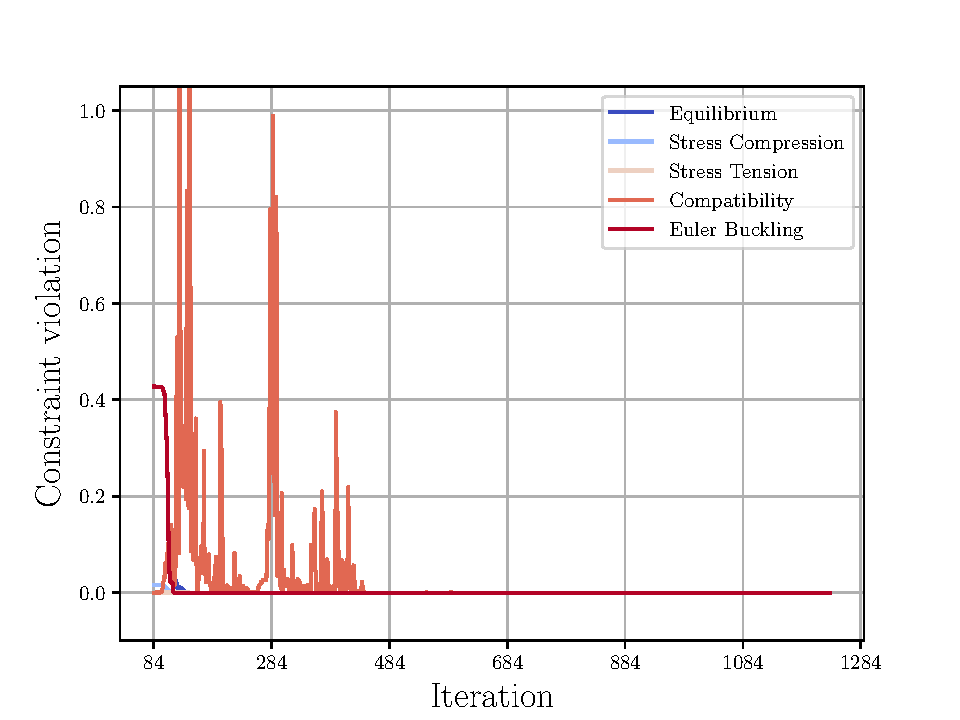
\includegraphics[width=0.49\linewidth]{figures/07_aeronautic/19b_c_hist_315.pdf}}
        \caption{Iteration history of the CRM-315 test case solved with the 2S-5R algorithm. (a) objective function history for the SLP and NLP step. The sharp increases in the objective function during the SLP step correspond to the reinitialization calls. (b) constraint violation for the NLP step.}
        \label{fig:07_c2}
    \end{figure*}

\paragraph{Maximum displacements constraints}
The designer of a plane could be interested in limiting the maximum Z displacement $Z_{t,\ell}$ of the wing tip to avoid a too high flex on the wing that could influence too much the aerodynamic field attorno all ala. We remember that controlling the displacements of the structure, we can actively influence the complance of the structure, even if the compliance minimization is not in the objective function. Additionally, this could be a constraint that can passively add stiffness to the wing and helps with the aeroelastic phenomenon of flutter instability.

having observed that in the unconstrained version the maxiumm tip dispalcement of the optimized CRM-315 structure, that has a half wing span of \qty{29.4}{m}, is $Z_t=\qty{4.11}{m}$, we set three differet $Z_{t,\ell} = [\qty{1}{m},\qty{2}{m},\qty{3}{m}]$ in the \gls{nlp} step, willing to explore ho sensible is the optimized structure is with respect to this constraint. The optimization are efectuated using the same material, geometrical and load data used in the above example.

\begin{table}
    \small
    \centering
    \begin{tabular}{ccccc}
    \toprule
    $\bm{Z}_{t,\ell}\:[\text{m}]$ & 1&2&3&--\\ \midrule
    V [\unit{\meter^3}]&  26.70&13.78&9.39&7.90\\
    V [\unit{\%}]&   \qty{4.421}{\%}   & \qty{2.283}{\%}&\qty{1.556}{\%}&\qty{1.309}{\%}  \\
    Mass [\unit{\tonne}]  &72.086&37.218&25.363&21.342\\
    a$_{\text{max}}$ [\unit{\meter^2}]&  0.615    & 0.293&0.197&0.198\\
    C$_\text{LC\_1}$ [\unit{\mega \joule}]   &  1.05    &  1.96&2.79& 3.23\\
    C$_\text{LC\_2}$ [\unit{\mega \joule}]   &   0.37   &  0.71&1.04& 1.28\\
    C$_\text{LC\_3}$ [\unit{\mega \joule}]   &   0.26   &  0.47&0.67& 0.76\\

    \bottomrule
    \end{tabular}
    \caption{remember \todo{put here the span of the wing}}
    \label{tab:07_disp}
\end{table}

\begin{figure*}
    \centering
    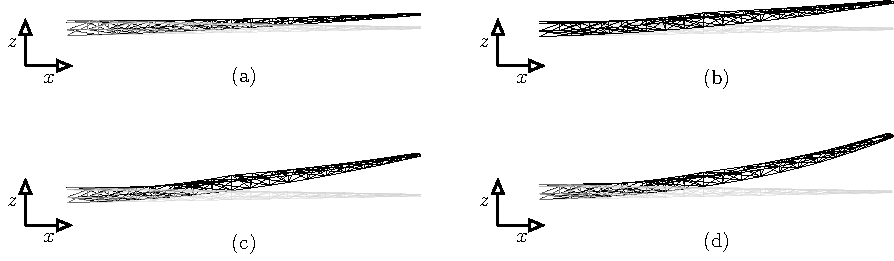
\includegraphics[width=\linewidth]{figures/07_aeronautic/00_dispalcements/disp.pdf}
     \caption{Undeformed (gray) and deformed (black) shapes of the optimized CRM-315 structures with half wing span of \qty{29.4}{m} for different values of maximum Z displacement $Z_{t,\ell}$ of the wing tip constrints. (a) $Z_{t,\ell}=\qty{1}{m}$  ; (b) $Z_{t,\ell}=\qty{2}{m}$; (c) $Z_{t,\ell}=\qty{3}{m}$; (d) no maximum displacement constraints.}
    \label{fig:07_disp_sol}
\end{figure*}

We plot the displacements in the XZ plane in \figref{fig:07_disp_sol} and the numeric values of the optimization in \tabref{tab:07_disp}. First, we notice how efficacely the optimizer limited the maximum displacement and converged to a solution even with a hard to satisfy constraint as $Z_{t,\ell}=\qty{1}{m}$ \marginnote{We remember that the \gls{crm} shows a half wing span of \qty{29.4}{m}.} . Second, we see that the constraint satisfaction doesent come free. The added rigidity needed to comply with the maximum displacement constraint come from a massive add of material that represent a \qty{19}{percent}, \qty{75}{percent} and \qty{237}{percent} increase for the $Z_{t,\ell} = [\qty{3}{m},\qty{2}{m},\qty{1}{m}]$, rispectively. Finally, as already stated before, the constaints on the maximum displacements infuence a lot the compliance of the structure, and we can see how, even if the proposed formulation does not keep into account for that, we can reduce indrecly the compliance of the structure.

\paragraph{Multiple materials}
The proposed formulation uses the material data as an input for the optimization and up untill this point we never interested in seeing how the mateial data could influence the topology and the final volume of the optimized structure. However we know how much the material is important and we wnat here see the influence on the CRM-315 test case. 

\begin{table}
    \small
    \centering
    \begin{tabular}{ccccc}
    \toprule
    \textbf{Material} &\textbf{Aluminium}&\textbf{Titanium}&\textbf{Steel}&\textbf{Pultruted CFRP}\\ \midrule
    $E$& \qty{69}{GPa}&\qty{120}{GPa}&\qty{210}{GPa}&\qty{150}{GPa}     \\
    $\sigma_\text{c}, \sigma_\text{t}$ & $\pm $\qty{270}{MPa}&$\pm $\qty{880}{MPa}&$\pm $\qty{355}{MPa}&+1200,\qty{-880}{MPa} \\
    $\rho$& \qty{2.7}{\gram\per\cubic\centi\metre}&\qty{4.5}{\gram\per\cubic\centi\metre}&\qty{7.8}{\gram\per\cubic\centi\metre}&\qty{1.6}{\gram\per\cubic\centi\metre}   \\
    \unit{kg CO^2_e\per\kilo\gram}&12.5&47.0&5.0&34.5 \\
    \unit{\$\per\kilo\gram}&2.2&23.5&6.3&40.5\\
    \bottomrule
    \end{tabular}
    \caption{remember \todo{put here the span of the wing}}
    \label{tab:07_materials_data}
\end{table}

We used four different materials commonly used in the aerospace domain: an alluminium alloy, titanium alloy, inox steel and pultruted \gls{cfrp}, of which mecanical properties are reported in \tabref{tab:07_materials_data}. on the top of classic material properties as young modulus, yeld stress and density we also take into account the enviromental cost \ie the mass of equivalent co2 emitted to produce a unit mass of the material and also the economic cost in dollar. We took this value from the book of Ashby \sidecite{ashby_materials_1999}. 

\begin{table}
    \small
    \centering
    \begin{tabular}{ccccc}
    \toprule
    \textbf{Material} &\textbf{Aluminium}&\textbf{Titanium}&\textbf{Steel}&\textbf{Pultruted CFRP}\\ \midrule
    V [\unit{\meter^3}]&7.90&4.53&5.88&3.67\\
    V [\unit{\%}]&\qty{1.309}{\%}&\qty{0.749}{\%}&\qty{0.974}{\%}&\qty{0.607}{\%}\\
    Mass [\unit{\tonne}]& 21.342&20.372&46.168&5.868\\
    a$_{\text{max}}$ [\unit{\meter^2}]&0.198&0.088&0.153&0.086\\
    C$_\text{LC\_1}$ [\unit{\mega \joule}]&3.23&4.88&1.33&4.39\\
    C$_\text{LC\_2}$ [\unit{\mega \joule}]&1.28&1.94&0.53&1.73\\
    C$_\text{LC\_3}$ [\unit{\mega \joule}]&0.76&1.15&0.31&1.03\\
    $Z_t\:[\text{m}]$&4.10&5.97&1.70&5.31\\
    Cost [\unit{\tonne CO^2_e}]&266.7&957.5&230.8&202.4\\
    Cost [\unit{k\$}]&46.9&478.7&290.8&237.6\\
    \bottomrule
    \end{tabular}
    \caption{remember \todo{put here the span of the wing}}
    \label{tab:07_materials}
\end{table}

The numerical results are presented in \tabref{tab:07_materials} and different observation can be made. First, we confirm that the mass of the optimized structure is highly influenced by the material choice, and more exactly it seems particularry influenced by the specific resistance and specific stiffness of the material. Second we notice that also the value of the complance and the maximum tip displacement is very influenced by material data, and more exactly elle est pilotée par le rapport entre strenght and young modulus of the material. This because with a material more strong we have smaller cross sectionals areas and thus smaller global rigidity. Third, is the volume behaviour, that follows a hyperbolic law with respect to the strenght of the material (as in this specific case the most volumic elements are constraint by stress and not buckling, see the constraints analysis later in the chapter). We finally give the deformed structuresi in \figref{fig:07_mat_sol}, in wich we claerly see how the titanium and the pultruted cfrp shows high deform shapes due to their high material properties.

We then observe the environmental and economic cost of the 4 structures. having a look at \figref{fig:07_cost}, we notice how, a part from titanium, the structures shows almost the same environmental cost for the production of the material. this come as unexpected due to the very different spectific c02 emission \eg there is a difference of almost 7 times between steel and CFRP. However the cfrp solution shows a massively reduction in weight that at the end favours it with respect to steel and even aluminum. A similar result can be observed in cost, anche se the very low production cost favors aluminum with respect to all other materials. It seems that at the end for this specific load case, the CFRP, even if costing more than aluminium, represent the better compromise between excellent mechanical properties, environmental and economic cost. Finally, ovviamente qui si tiene in conto solo del costo del materiale, ma il peso inferiore su un aero permette di risparmiare veramente molto di piu rispetto al costo della sola produzione. questo favorisce ancora di piu il caso pultruted CFRP.

\begin{figure*}
    \centering
    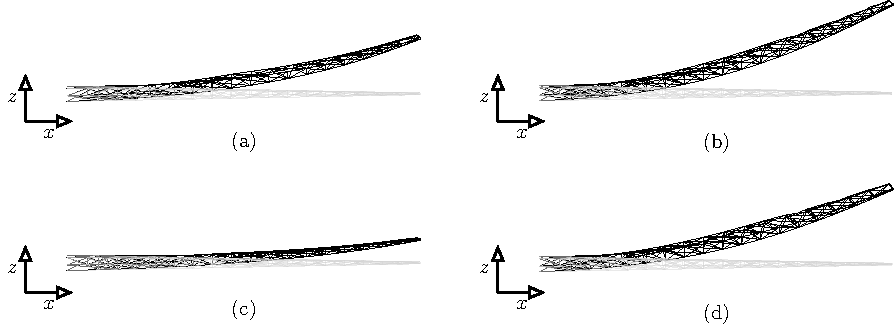
\includegraphics[width=\linewidth]{figures/07_aeronautic/00_materials/mat.pdf}
     \caption{}
    \label{fig:07_mat_sol}
\end{figure*}

\begin{marginfigure}
    \centering
    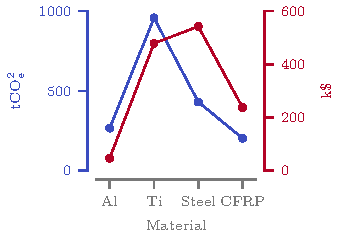
\includegraphics[width=\linewidth]{figures/07_aeronautic/00_co2eq/co2_dollar.pdf}
    \caption{}
    \label{fig:07_cost}
\end{marginfigure}

\paragraph{Enriching the mesh}
As earlier described in the chapter, we want now to assess the influence of the initial ground structure on the volume and topology of the optimized structure. We use then the refined ground structure called CRM-2370, optimized for the smae threee load cases used precedently and using the aluminium as material.

\begin{figure*}
    \centering
    \includegraphics[width=\linewidth]{figures/07_aeronautic/16_wing_opt/wing_opt.pdf}
     \caption{Maximum stress constraint value (left) and buckling constraint value (right) plotted on the deformed shape of the optimized design (undeformed shape in light grey) of CRM-2370 for the three load cases: +2.5 g maneuver (a), -1 g maneuver (b), and cruise with gust (+1.3 g) (c). The maximum $z$ tip deflection is \qty{4.167}{m}, \qty{-2.953}{m}, and \qty{1.948}{m}, respectively.}
    \label{fig:07_wing_opt}
\end{figure*}
The mass of the optimized CRM-2370 structure is \qty{20.092}{\tonne}, a \qty{1.318}{\tonne} reduction compared to the CRM-315 (\qty{-6.2}{\%}). Additionally, if we compare the compliance of the three load cases (see \tabref{tab:07_wing-res}), we notice how the solution of CRM-2370 is not only lighter but also stiffer, suggesting in general a more efficient structure topology. The maximum \todo{[sostituiscci con Zell]} z tip deflection of the wingbox is \qty{4.167}{m}, \qty{-2.953}{m}, \qty{1.948}{m} for the three considered load cases, respectively. There are 1127 active bars in the optimized design, and the whole optimization took \qty{3189}{s} (\qty{1911}{s} for the \gls{slp} step, \qty{1278}{s} for the \gls{nlp} step). The iteration history curves of the optimization are plot in \figref{fig:07_c3}. In \figref{fig:07_wing_opt} the normalized maximum stress and buckling constraints are plotted on the deformed shape of the three load cases. We notice how in general the topology of the two external "spars" is shaped after the +2.5 g load case, while the interior of the wingbox is made by a thinner truss constrained by buckling. 

\begin{figure*}
    \centering
    \subcaptionbox{}{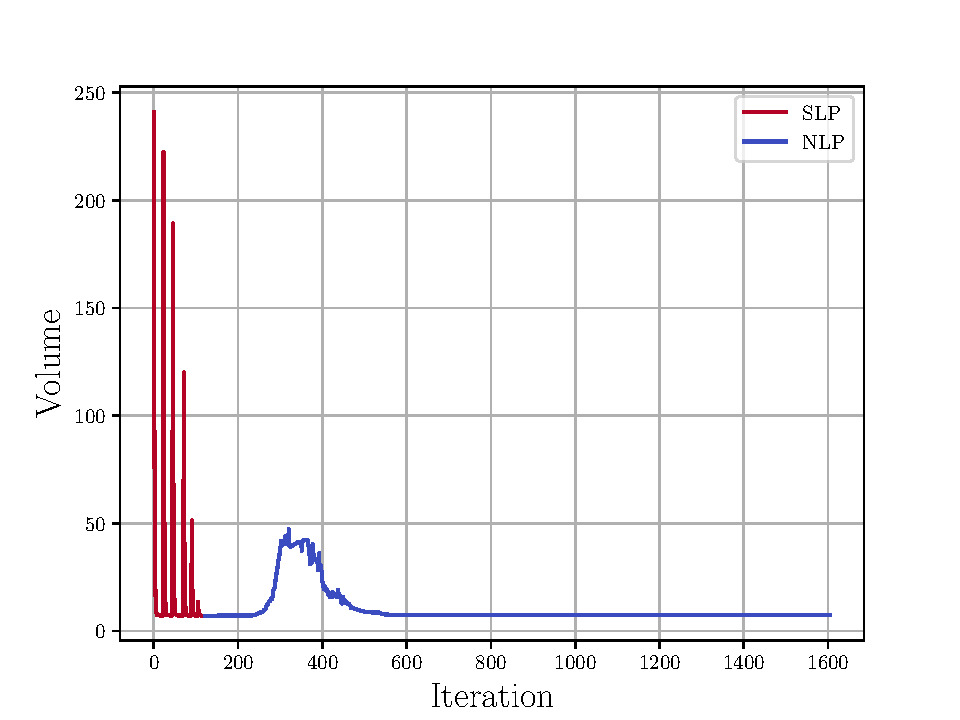
\includegraphics[width=0.49\linewidth]{figures/07_aeronautic/20a_v_hist_2370.pdf}}
    \bigskip
    \subcaptionbox{}{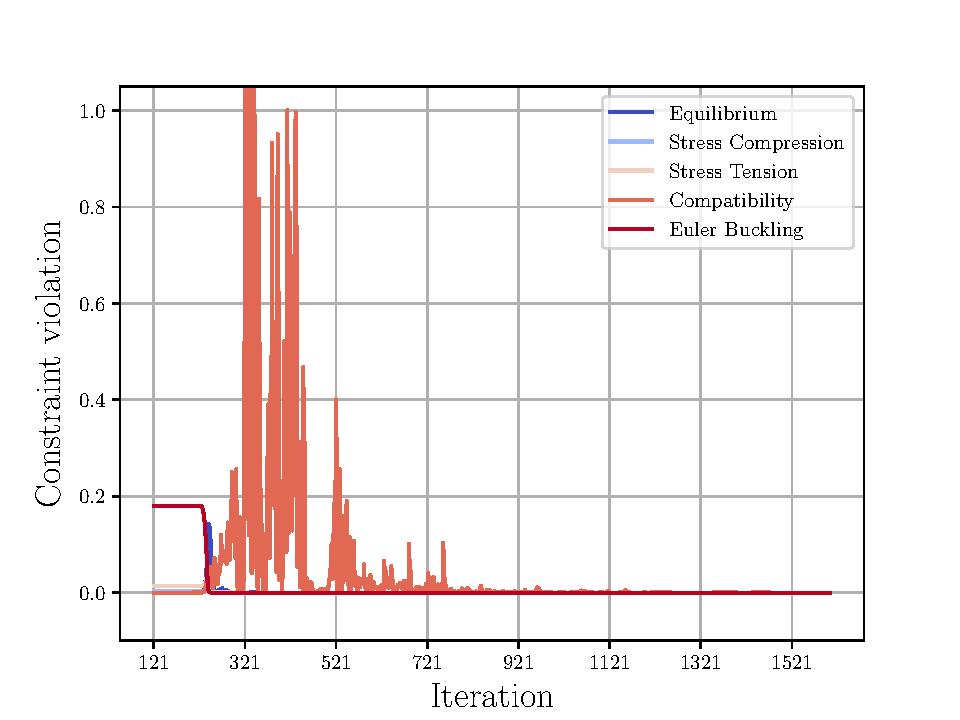
\includegraphics[width=0.49\linewidth]{figures/07_aeronautic/20b_c_hist_2370.pdf}}
    \caption{Iteration history of the CRM-2370 example solved with the 2S-5R algorithm. (a) objective function history for the SLP and NLP step. The sharp increases in the objective function during the SLP step correspond to the reinitialization calls. (b) constraint violation for the NLP step.}
    \label{fig:07_c3}
\end{figure*}

\paragraph{Active mechanical constraints}
To better understand which mechanical phenomena is the most constraining for the bars of the solution, we present in \figref{fig:fail-crm} a graph where the normalized stress criterion $\vect{c_s}=\max{\left(-\vect{q} \; \textit{\textbf{sf}}/\sigma_c \vect{a},\vect{q} \; \textit{\textbf{sf}}/\sigma_t \vect{a}\right)}$ and the normalized buckling criterion $\vect{c_b}=\vect{q}\; \textit{\textbf{sf}}/\vect{q}_{\text{crit}}$ are plotted against each other. Every point in the scatter plot represents the members of the solution of the \gls{slp} and the \gls{nlp} steps that show at least a charge of 1N (931 out of 1127 members). This threshold is applied as at the end of the NLP step some members present a very small section, creating numerical problems when evaluating the stress and buckling criteria. All the \gls{slp} members activate either the maximum stress or buckling limit, while 68 out of 931 \gls{nlp} members are located in the center of the graph ($c_s<0.95$ and $c_b<0.95$). We speculate that this behavior is due to the inclusion of the kinematic compatibility constraint in the \gls{nlp} algorithm: the cross-sectional area of these bars is chosen to comply with the global displacements. In \tabref{tab:07_constrNLP}, a summary of the active mechanical failure constraints (buckling, tensile stress, and compressive stress) present in the NLP solution. The table showcases the number of active constraints categorized by constraint type and load case. The optimized design encompasses a total of 930 active mechanical failure constraints for 863 bars (931 minus the 68 bars constrained by kinematic compatibility). This suggests that certain members are concurrently subject to multiple failure constraints across different load cases. An additional observation is that the design of the solution is primarily influenced by local buckling and compressive failures, especially under the +2.5 g load case (LC\_1).

\begin{figure}
    \centering
    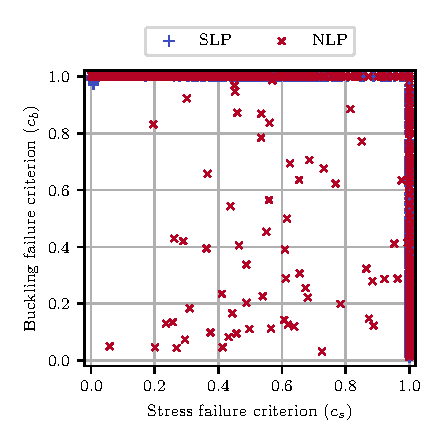
\includegraphics[width=0.8\linewidth]{figures/07_aeronautic/18_failure new/failure_max.pdf}
     \caption{Normalized buckling and maximum stress constraint values for the optimized CRM-2370 structure after the SLP and the NLP optimization steps.}
    \label{fig:fail-crm}
\end{figure}

\begin{table}
\small
\centering
\begin{tabular}{lS[table-format=3.0]S[table-format=3.0]S[table-format=3.0]S[table-format=3.0]S[table-format=3.0]}
\toprule
                     & \textbf{LC\_1} & \textbf{LC\_2} & \textbf{LC\_3} & \textbf{Tot.} \\ \midrule
\textbf{Buckling}    & 281           & 145           & 143           & 569           \\
\textbf{Tension}     & 56            & 3             & 4             & 63            \\
\textbf{Compression} & 286           & 6             & 6             & 298           \\
\midrule
\textbf{Tot.}        & 623           & 154           & 153           & 930          \\
\bottomrule
\end{tabular}
\caption{Number of active mechanical failure constraints for the CRM-2370 optimized design per type of constraint (rows) and per load case (columns).}
\label{tab:07_constrNLP}
\end{table}

\section{NACA 0012 modular drone wing}
\begin{figure}
    \centering
    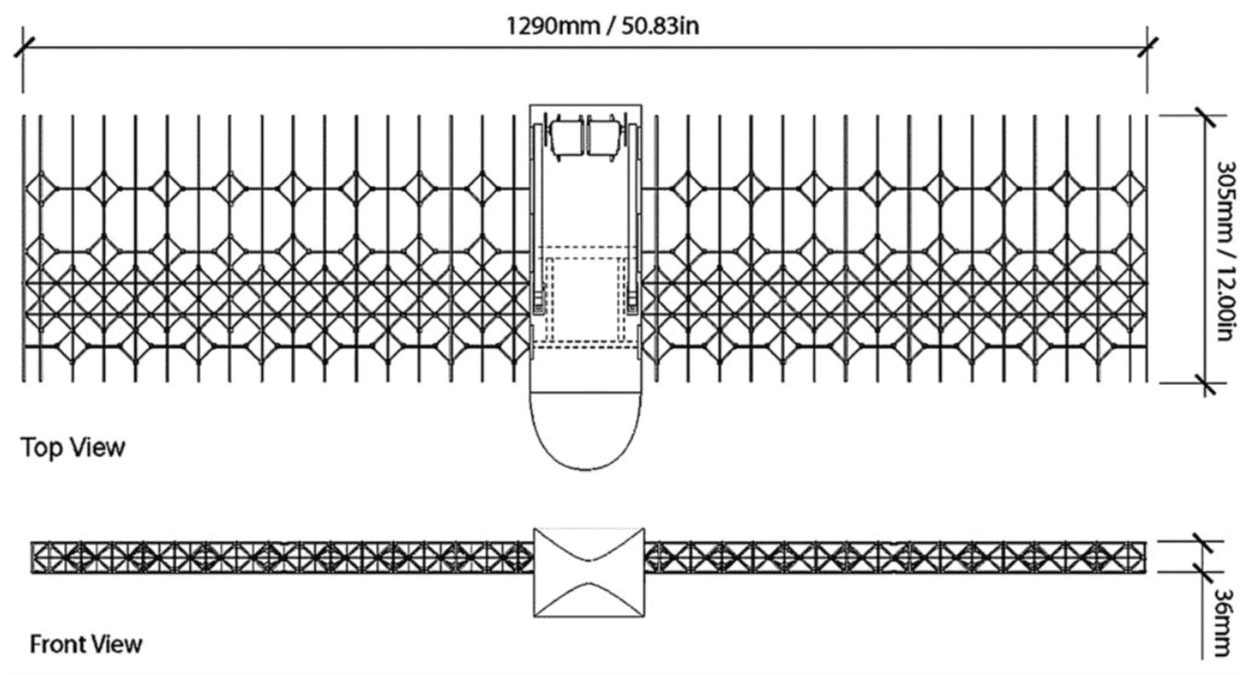
\includegraphics[width=0.8\linewidth]{figures/07_aeronautic/naca0012.png}
        \caption{ \cite{jenett_digital_2017}}
    \label{fig:07_naca0012}
\end{figure}
We will now deal wit another aeronautical test case. One of the possible and most fitting application for modular structures is the use for small fixed wing drones. THis because of the easy in field deployement, easy to repair structure and extreme lightweight. Jenett and his working group at NASA developed an experimental platform for the study of active morphing wings using lattices which dimensions are shown in \figref{fig:07_naca0012}. The platform wing volume is obtained by extruding by $b=\qty{580}{mm}$ a NACA 0012 airfoil with a chord $c=\qty{305}{mm}$. We are taking the exact same volume for our modular optimization, and instead of focussing on aerodynamic and aeroelastic properties, we deal with the optimization of the internal structure. As the platform was not meant for flying, the authors dont share additional data on the requirement used to design the internal structure. For that reason, we assume in a conservative way a $\text{MTOW}=\qty{10}{kg}$ and we design the structure to withstand a maximum loading factor $\text{nz}=2$.
\begin{margintable}
    \small
    \centering
    \begin{tabular}{cc}
    \toprule
    \textbf{Parameter}        & \textbf{Value} \\ \midrule
    $E$              & \qty{6.8}{GPa}     \\
    $\sigma_\text{c}, \sigma_\text{t}$ & $\pm $\qty{140}{MPa} \\
    $\rho$              & \qty{1.42}{\gram\per\cubic\centi\metre}   \\
    \bottomrule
    \end{tabular}
    \caption{Material data of the Ultem 2200 used for the NACA 0012 optimization.}
    \label{tab:07_NACA_mat}
\end{margintable}
As the wing present a rectangular planform on the XY plane we assume a constant lift distribution on the X axis (span of the extruded profile). as a further simplification, we assume the lift distrubutiion as constant also on the Y plane (chord plane). THe lift distribution is then integrated to evaluate the concentrated nodal load necessary to conduct our optimization. In this settings all the nodes on the upper skin are then equally loaded in the Z direction. As already done in the \gls{crm} test case, we dont take into account the effect of the skin on the mechanical model. Finally, the material used for the optimization is the Ultem 2200, a high-performance thermoplastic material filled at \qty{20}{\percent} by glass fiber and known for its exceptional strength, heat resistance, chemical resistance, and suitability for applications requiring durability. Thei mecahnical properties are summarized in \tabref{tab:07_NACA_mat}.

\subsection{Modular ground structure generation for irregular volumes}
Compared to the academic test cases presented in \chpref{chap:05} and \chpref{chap:06}, the extruded NACA 0012 profile does not present a regular parallepipedic shape that is easily partitioned in cubic subdomains. The easiest solution in this particular scenario of the extruded wingfoil case would be to partition the structure in sections by performing multiple cutting on the YZ plane, but this strategy woul not apply to more complex external shapes. For that reason we developed a ground structure generation strategy that maximizes the generation of modular domains on complex volumes. First, we generate a cloud of nodes equally repartitioned in the trhee axis. The distance between nodes on the three axis represent an hyperparameter for the user that could via this parameter chose the size of the geometry of the repeating module. All these phases are presented grphically on \figref{fig:07_howto}.

\begin{figure*}
    \centering
    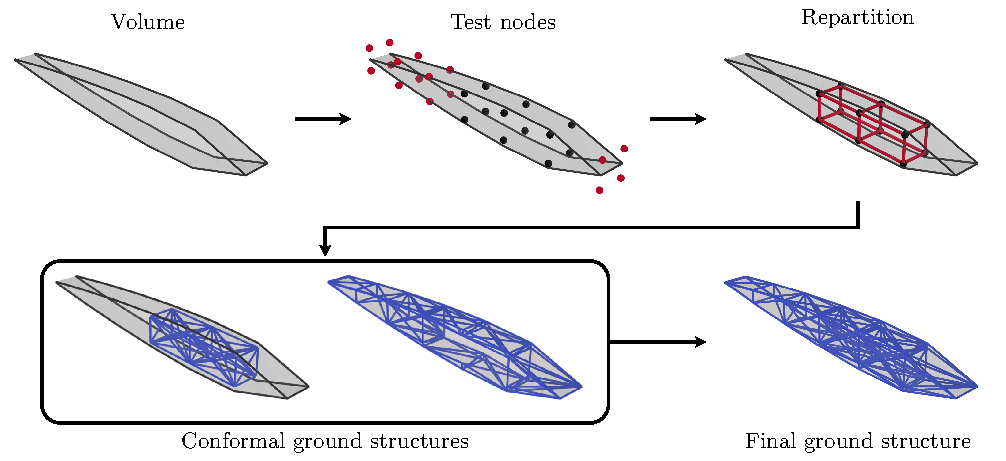
\includegraphics[width=\linewidth]{figures/07_aeronautic/00_naca_howtomesh/MESH.pdf}
     \caption{}
    \label{fig:07_howto}
\end{figure*}

\subsection{Numerical optimization of the modular NACA 0012 drone wing}
\todo{BC}

\begin{figure*}
    \centering
    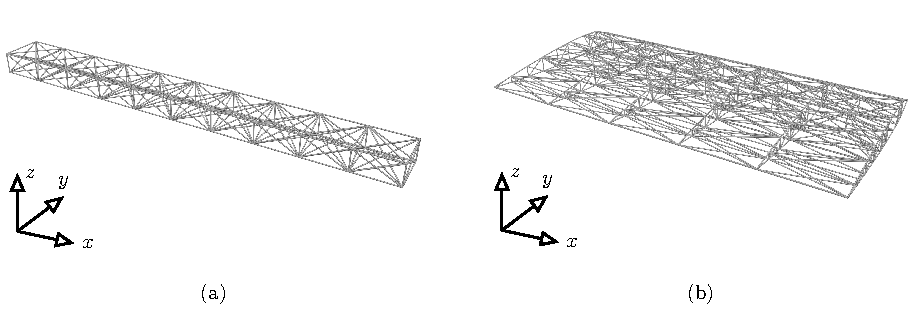
\includegraphics[width=\linewidth]{figures/07_aeronautic/00_NACA_a_gs_cell/gs_a_types.pdf}
     \caption{}
    \label{fig:07_}
\end{figure*}

\begin{figure*}
    \centering
    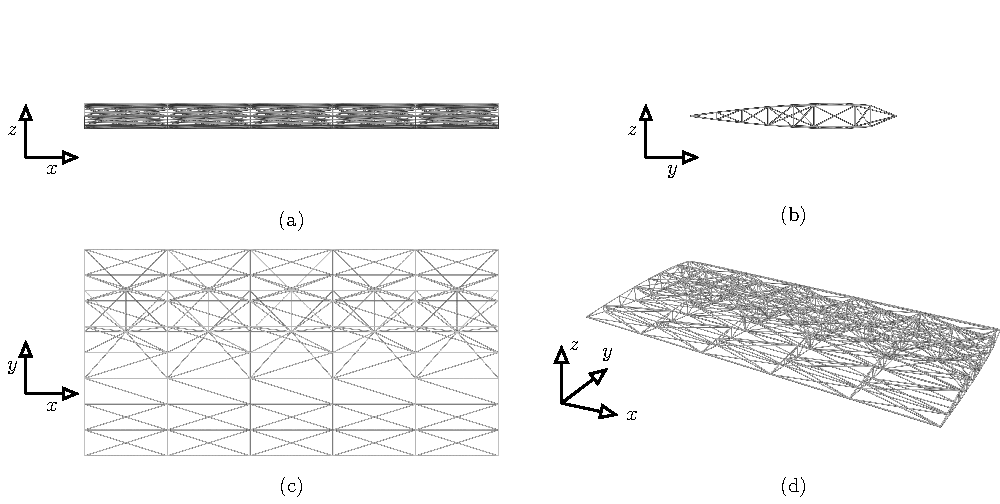
\includegraphics[width=\linewidth]{figures/07_aeronautic/00_NACA_gs/gs_a.pdf}
     \caption{}
    \label{fig:07_}
\end{figure*}

\begin{figure*}
    \centering
    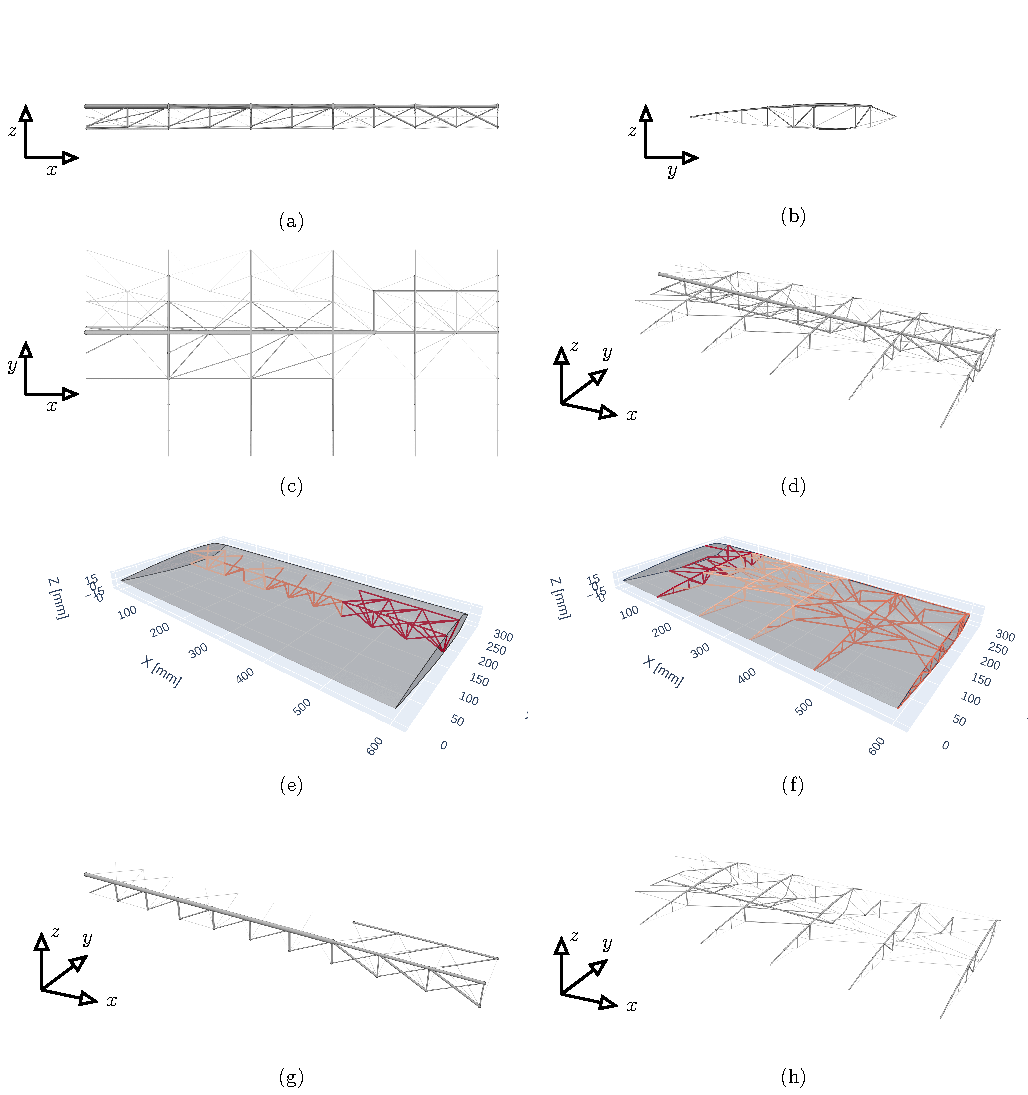
\includegraphics[width=\linewidth]{figures/07_aeronautic/00_NACA_a_sol_3/gs_a.pdf}
        \caption{}
    \label{fig:07_}
\end{figure*}

\begin{figure}
    \centering
    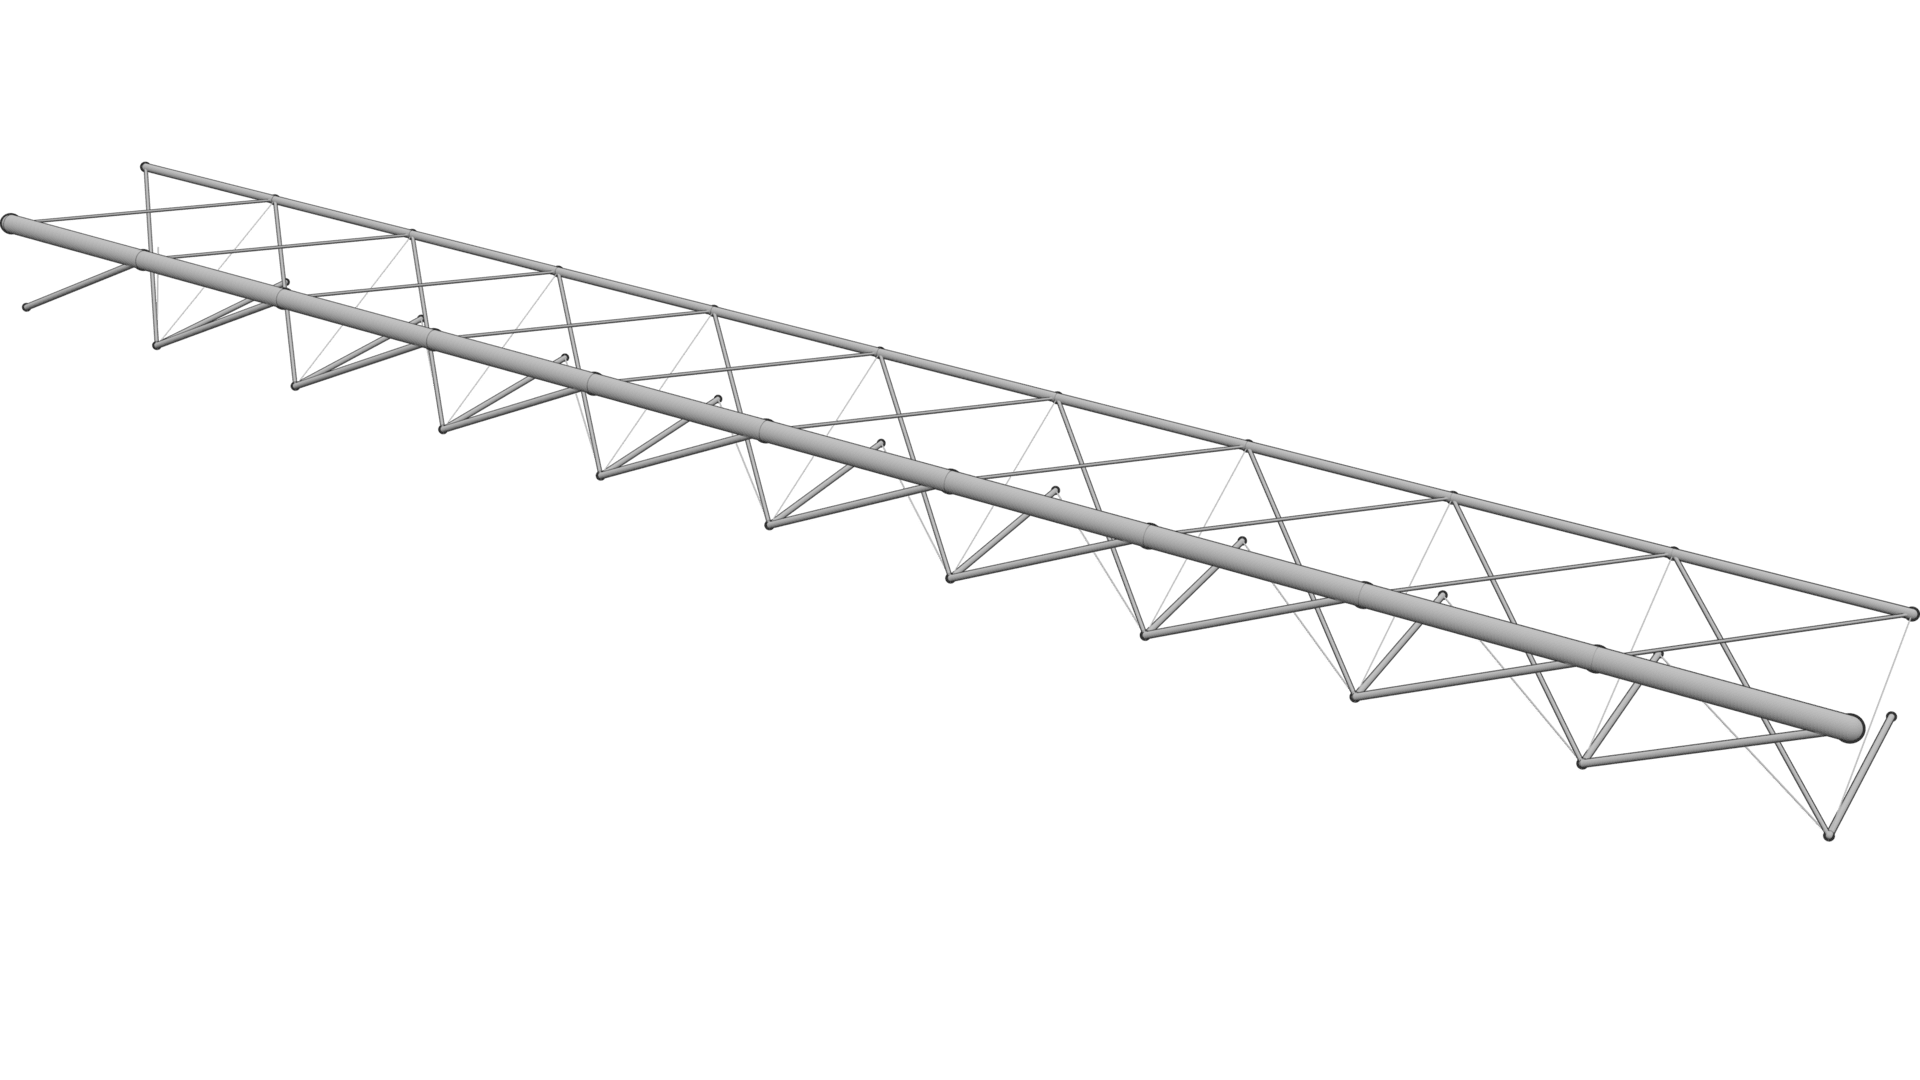
\includegraphics[width=0.8\linewidth]{figures/07_aeronautic/00_NACA_c_1/04_Topology_cell_iso.png}
        \caption{}
    \label{fig:07_}
\end{figure}

\begin{figure}
    \centering
    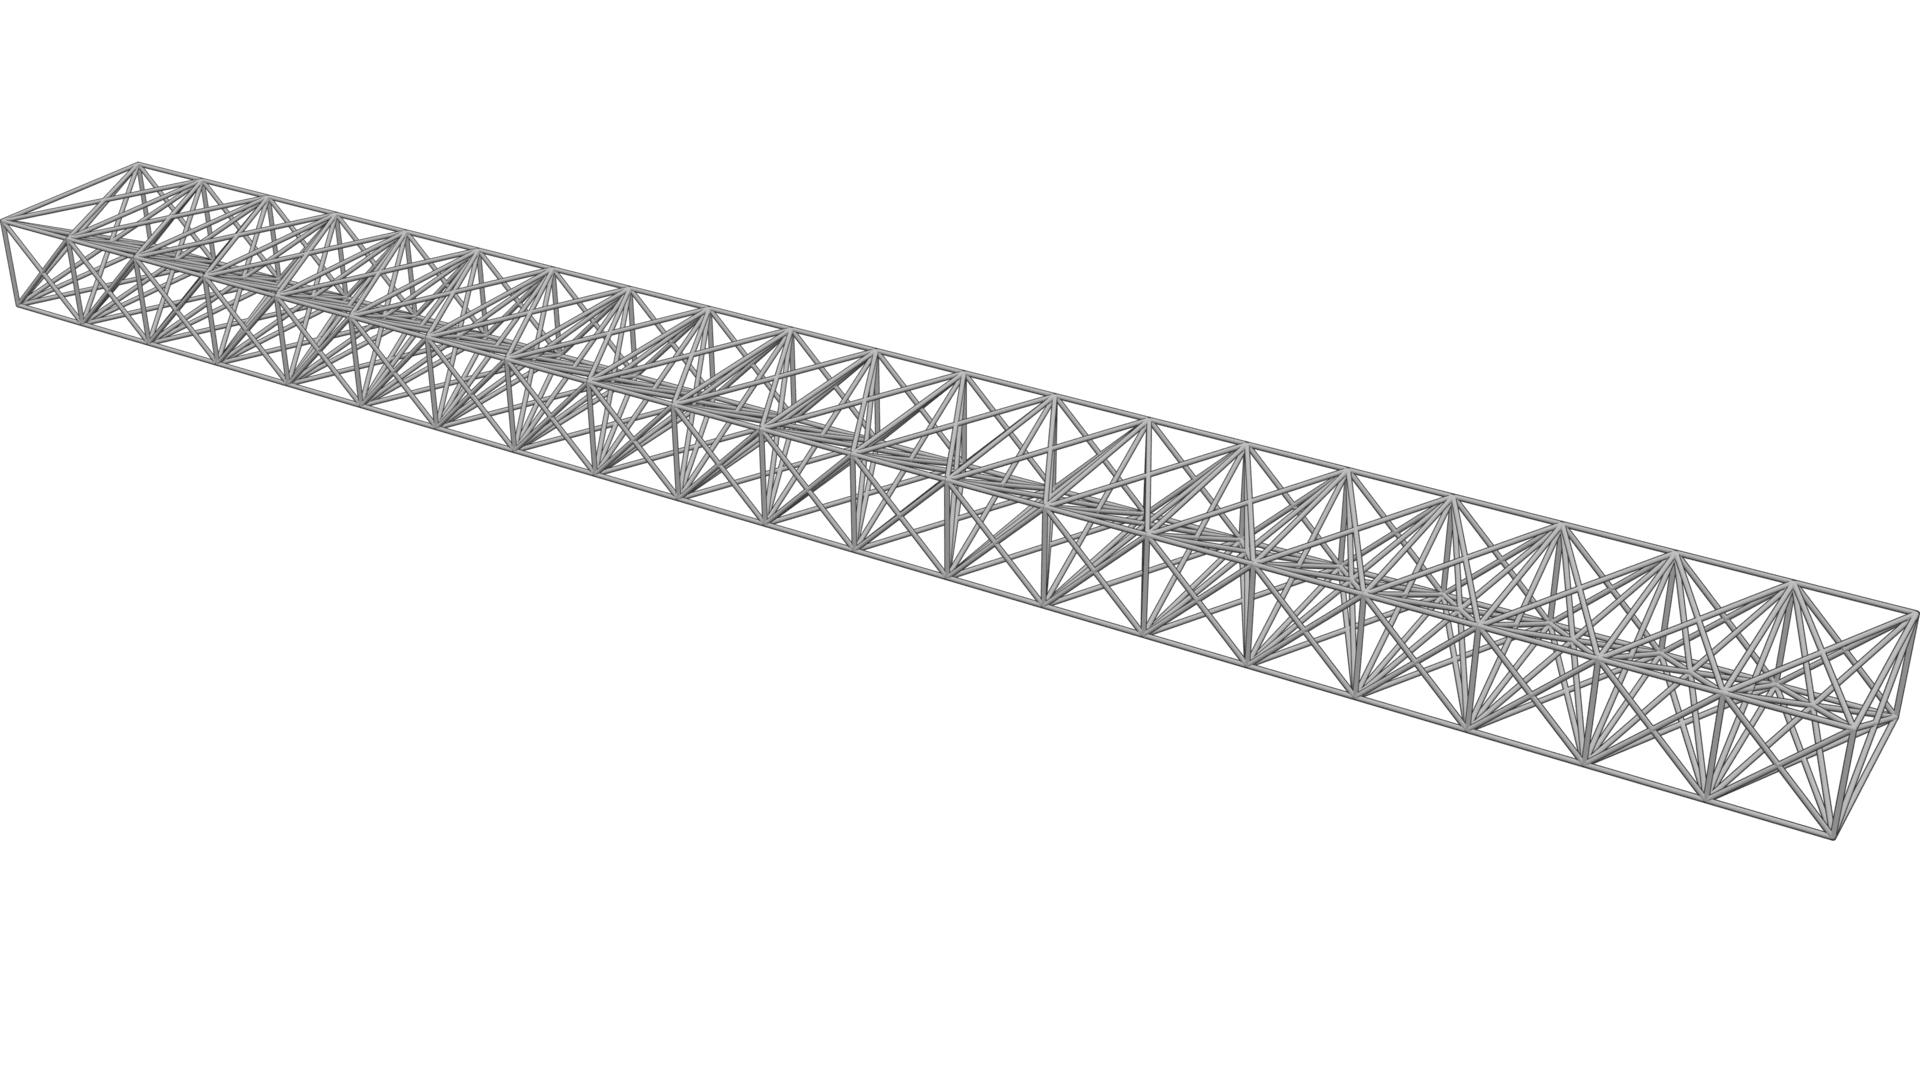
\includegraphics[width=0.8\linewidth]{figures/07_aeronautic/00_NACA_gs_b/02_GS_c_iso.png}
        \caption{}
    \label{fig:07_}
\end{figure}

\begin{marginfigure}
    \centering
    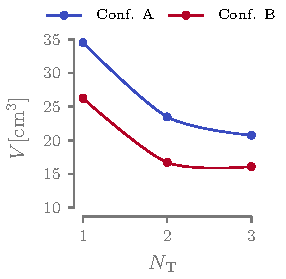
\includegraphics[width=\linewidth]{figures/07_aeronautic/00_NACA_vol_crv/vol.pdf}
    \caption{}
    \label{fig:07}
\end{marginfigure}

\begin{figure*}
    \centering
    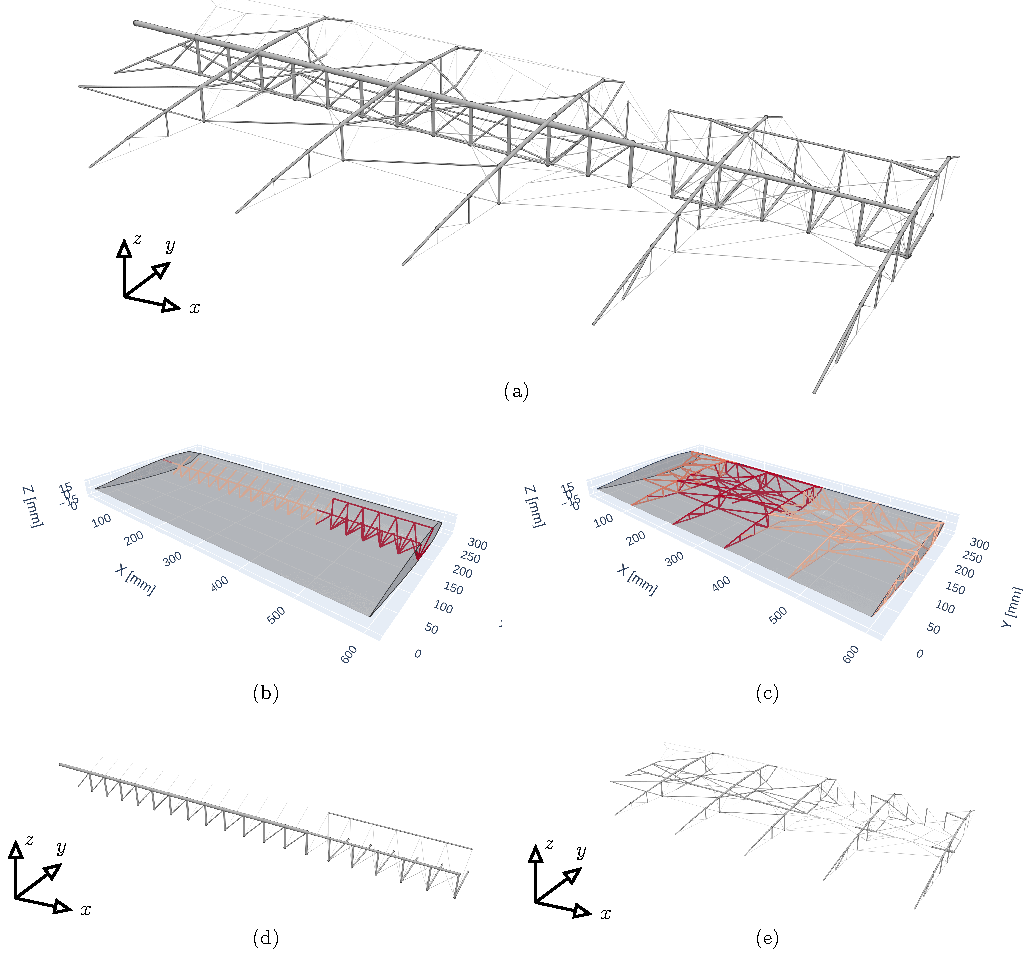
\includegraphics[width=\linewidth]{figures/07_aeronautic/00_NACA_b_sol_3/gs_a.pdf}
        \caption{}
    \label{fig:07_}
\end{figure*}

\begin{table*}
    \centering
    \small
    \begin{tabular}{lx{1.4cm}x{1.4cm}x{1.4cm}x{1.4cm}x{1.4cm}x{1.4cm}}
        \toprule
         &\multicolumn{3}{l}{Configuration A} & \multicolumn{3}{l}{Configuration B} \\ 
             \cmidrule(lr){2-4} \cmidrule(lr){5-7} 
    $N_\text{T}$&1&2&3&1&2&3\\
    $N_\text{opt}\;(N_\text{el})$ & 425 (1155)&503 (1155)& 366 (1155)&620 (1675)&539 (1675)&454 (1675) \\
    Mass [\unit{g}]&49.0&33.3&29.5&37.3&23.8&22.9 \\
    $V$ [\unit{\percent}] &0.81&0.55 &0.48&0.62&0.39&0.37        \\
    $\bar{\rho}$ [\unit{kg/m^3}] &11.53&7.84&6.93&8.76&5.59&5.38\\
    $\varphi$    &\qty{22.5}{\percent}&\qty{37.9}{\percent}&\qty{56.0}{\percent}&\qty{19.0}{\percent}&\qty{36.9}{\percent}&\qty{50.0}{\percent} \\
    $\psi$    &0.45&0.69&0.73&0.46&0.70&0.72\\ 
    t        & \hms{0;0;39}  & \hms{0;5;6} & \hms{0;2;3} & \hms{0;2;28} & \hms{0;3;32}&\hms{0;5;1}\\
    \bottomrule
    \end{tabular}
    \caption{Numeric results of the parametric study on the influence of the number of modules $N_\text{T}$ on the NACA 0012 drone wing.}
    \label{tab:07}
    \end{table*}

\section{Conclusion}